\documentclass{beamer}

\usepackage{german}    %Block zum Setzen von Umlauten
\usepackage{lmodern}
\usepackage[utf8]{inputenc}

\mode<presentation>
\definecolor{hdaRot}{cmyk}{0,1,1,0.18}     % -5005
\definecolor{hdaBlauMed}{cmyk}{0.71,0.25,0,0}     % -1169
\definecolor{hdaGruenMed}{cmyk}{0.5,0.13,1,0.06}    % -2048

\setbeamercolor*{kred}{fg=hdaRot}
\setbeamercolor*{kblue}{fg=hdaBlauMed}
\setbeamercolor*{kgreen}{fg=hdaGruenMed}
\setbeamercolor*{kblack}{fg=black}
\setbeamerfont{block body alerted}{size=\huge}
\setbeamerfont{block title alerted}{size=\huge}
\setbeamercovered{transparent=25}
\usebeamercolor{normal text}
\mode<all>

\newcommand{\hlblue}{%
\usebeamercolor[fg]{normal text}%
\only{\usebeamercolor[fg]{kblue}}}

\newcommand{\hlgreen}{%
\usebeamercolor[fg]{normal text}%
\only{\usebeamercolor[fg]{kgreen}}}

\newcommand{\hlblack}{%
\usebeamercolor[fg]{normal text}%
\only{\usebeamercolor[fg]{kblack}}}

\newcommand{\hlred}{%
\usebeamercolor[fg]{normal text}%
\only{\usebeamercolor[fg]{kred}}}

\usepackage{tikz}
\usetikzlibrary{calc}

\usetikzlibrary{arrows,decorations.pathmorphing,backgrounds,positioning,fit,petri}%

\makeatletter
\tikzset{pics/named scope code/.style={code={\tikz@fig@mustbenamed%
  \begin{scope}[local bounding box/.expanded=\tikz@fig@name]#1\end{scope}%
}}}
\makeatother

\tikzset {
  pics/p8way/.style n args = {8}{
    named scope code = {
      \draw (-3,-1.5) rectangle  (3, 1.5);
      \draw[line width=1pt]  (-3,-0.5) -- ( 3,-0.5);
      \draw[line width=1pt]  (-3, 0.5) -- ( 3, 0.5);
      \draw[line width=1pt]  (-1,-1.5) -- (-1, 1.5);
      \draw[line width=1pt]  ( 1,-1.5) -- ( 1, 0.5);

      \foreach \x / \y / \label in {
       -2/1/#1, 1/1/#2,
       -2/0/#3, 0/0/#4, 2/0/#5,
       -2/-1/#6, 0/-1/#7, 2/-1/#8
      }{\draw (\x,\y) node{\textbf{\label}};}
    }
  }
}

\begin{document}

\begin{frame}[t,shrink=65]
  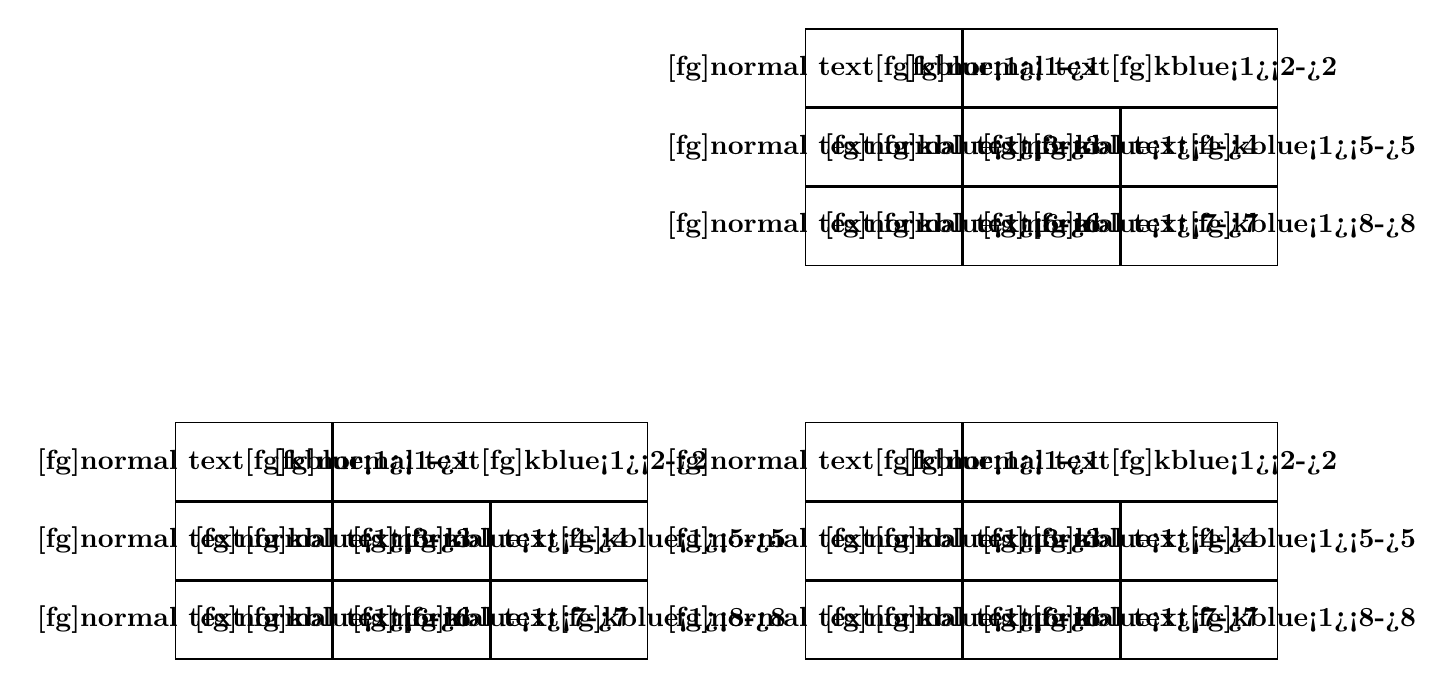
\begin{tikzpicture}
    \pic (N01) at (0,0) {p8way=%
      {\hlblue<1>\visible<1->1}
      {\hlblue<1>\visible<2->2}
      {\hlblue<1>\visible<3->3}
      {\hlblue<1>\visible<4->4}
      {\hlblue<1>\visible<5->5}
      {\hlblue<1>\visible<6->6}
      {\hlblue<1>\visible<7->7}
      {\hlblue<1>\visible<8->8}
    };
    \pic (N02) at (8,0) {p8way=%
      {\hlblue<1>\visible<1->1}
      {\hlblue<1>\visible<2->2}
      {\hlblue<1>\visible<3->3}
      {\hlblue<1>\visible<4->4}
      {\hlblue<1>\visible<5->5}
      {\hlblue<1>\visible<6->6}
      {\hlblue<1>\visible<7->7}
      {\hlblue<1>\visible<8->8}
    };
    \pic (N03) at (8,5) {p8way=%
      {\hlblue<1>\visible<1->1}
      {\hlblue<1>\visible<2->2}
      {\hlblue<1>\visible<3->3}
      {\hlblue<1>\visible<4->4}
      {\hlblue<1>\visible<5->5}
      {\hlblue<1>\visible<6->6}
      {\hlblue<1>\visible<7->7}
      {\hlblue<1>\visible<8->8}
    };

  \end{tikzpicture}
\end{frame}
\end{document} 